
\begin{table}[t]
\centering
%\scriptsize
%\resizebox{\columnwidth}{!}{
\begin{tabular}{|l|l|} \hline
\textbf{Application}& \textbf{Description}\\
\hline
Prophet& Time series decomposition and prediction\\ 
\hline
Multi-Regression& Multiple linear regression/prediction of time series\\
\hline
XGBoost& Regression and classification by gradient boosting\\
\hline
SVC & Classification based on support vector machine\\
\hline
NN& Classification by layered artificial neural network\\
\hline
\end{tabular}
%}
\caption{Machine learning applications used 
to evaluate Seneca. 
%paper submission is blind (so such references must be omitted so as not to reveal our identities):
%Code base is available at project repository~\cite{ref:seneca}.
\label{tab:bmarks}}
\vspace{-0.1in}
\end{table}

\begin{table}[t]
\centering
% \scriptsize
%\resizebox{\columnwidth}{!}{
\begin{tabular}{|l|l|l|} 
\hline
\textbf{Hyperparameter}& \textbf{Default} & \textbf{Tuning options}\\
\hline
growth & linear & [linear, logistic] \\
\hline
changepoint prior scale & 0.05 & [0.05, 0.5] \\
\hline
holidays prior scale & 10 & [1, 5, 10] \\
\hline
seasonality prior scale & 0.5 & [0.1, 0.5] \\
\hline
fourier order & 10 & [5, 10, 15, 20] \\
\hline
seasonality mode & additive & [additive, multiplicative] \\
\hline
interval width & 0.8 & [0.5, 0.8] \\
\hline
\end{tabular}
%}

\caption{Hyperparameters Seneca considers for \textbf{Prophet}. 
\label{tab:prophet_para}}
%\vspace{-0.1in}
\end{table}

\begin{table}[t]
\centering

\begin{tabular}{|l|l|l|} 
\hline
\textbf{Hyperparameter}& \textbf{Default} & \textbf{Tuning options}\\
\hline
%hidden layer size & 100 & [100] \\
%\hline
max depth & 3 & [3, 4]\\
\hline
learning rate & 0.1 & [0.1, 0.01] \\
\hline
N estimators & 100 & [100, 400] \\
\hline
objective & reg:linear & [reg:linear, rank:pairwise] \\
\hline
booster & gbtree & [gbtree, gblinear, dart] \\
%\hline
%n jobs & 1 & [1,4]\\
%\hline
%gamma & 0 & [0,0.01] \\
\hline
min child weight & 1 & [0.1, 1] \\
\hline
scale positive weight & 1& [1, 2] \\
%\hline
%sample tree & 1& [0.2,0.5,1]\\
%\hline
%samp level & 1& [0.2,0.5,1]\\
%\hline
%ralpha & 0& [0.0.1,0.9] \\
%\hline
%rlambda & 1& [0.1,0.9,1] \\
\hline
base score & 0.5 & [0.5, 10] \\
\hline
%random state & 123& [123] \\
%\hline
\end{tabular}

\caption{Hyperparameters Seneca considers for \textbf{XGBoost}. 
\label{tab:xgboost_para}}
\vspace{-0.2in}
\end{table}

\begin{table}[t]
\centering
%\scriptsize

\begin{tabular}{|l|l|l|} 
\hline
\textbf{Hyperparameter}& \textbf{Default} & \textbf{Tuning options}\\
\hline
C & 1.0 & [0.5, 1.0] \\
\hline
kernel & rbf & [rbf, linear, poly, sigmoid] \\
\hline
degree & 3 & [3, 4] \\
\hline
gamma & auto& [auto, scale] \\
\hline
coef0 init & 0.0 & [0.0, 1.0] \\
\hline
%shrink & True & [True] \\
%\hline
probability & False & [False, True] \\
\hline
tol & 1e-3& [1e-3, 1e-4] \\
\hline
%cache & 5.0& [5.0] \\
%\hline
%max iter & 20 & 20 \\
%\hline
decision function shape & ovr & [ovo, ovr] \\
\hline
%random state & 123& [123] \\
%\hline
\end{tabular}

\caption{Hyperparameters Seneca considers for \textbf{SVC}. 
\label{tab:svc_para}}
%\vspace{-0.2in}
\end{table}

\begin{table}[t]
\centering
%\scriptsize

\begin{tabular}{|l|l|l|} 
\hline
\textbf{Hyperparameter}& \textbf{Default} & \textbf{Tuning options}\\
\hline
%hidden layer size & 100 & [100] \\
%\hline
activation & relu & [identity, tanh, relu] \\
\hline
solver & adam & [lbfgs, sgd, adam] \\
%\hline
%alpha & 0.0001 & [0.0001] \\
%\hline
%batch size & auto & [200,auto] \\
\hline
learning rate & constant & [constant, invscaling, adaptive] \\
\hline
learning rate init & 0.001 & [0.001, 0.0001] \\
\hline
power T & 0.5 & [0.1, 0.5] \\
%\hline
%max iter & 20& [20] \\
%\hline
%shuffle & True& [True] \\
%\hline
%random & 123& [123] \\
\hline
tol & 1-e4 & [1e-4, 1-e5] \\
%\hline
%momentum & 0.9& [0.9] \\
%\hline
%early stop & False& [False] \\
%\hline
%beta1 & 0.9& [0.9] \\
%\hline
%beta2 & 0.999& [0.999] \\
%\hline
%epsilon & 1e-8& [1e-8] \\
\hline
n iter no change & 10 & [10, 20] \\
\hline
\end{tabular}

\caption{Hyperparameters Seneca considers for \textbf{NN}.
\label{tab:nn_para}}
\vspace{-0.2in}
\end{table}

In this section, we empirically evaluate Seneca in terms of machine learning (ML) 
model output quality, performance, and cost.
We first overview the ML applications 
that we consider and our experimental methodology. 
We then present our results. 

\subsection{Benchmark Applications and Training/Testing Datasets}
The ML applications that we use to evaluate Seneca 
are described in Table~\ref{tab:bmarks}.
Prophet, Multi-Regression, and XGBoost are regression
applications; 
XGBoost, SVC, and NN are classification applications (XGBoost 
implements both regression and classification tasks).
The regression applications compute the mean square error (MSE) 
as $\frac{1}{n}\sum_{i=1}^{n}(Y_i - \hat{Y_i})$, where $\hat{Y_i}$ is the ground truth, 
$Y_i$ is model prediction and n is the number of data points. The applications
return the average MSE across cross validations.
The classification applications compute and return a classification accuracy 
percentage, which is calculated
as $\frac{1}{n}\sum_{i=1}^{n}1(Y_i = \hat{Y_i})$, where $Y_i$ is the
prediction class, $\hat{Y_i}$ is the true class, $n$ is the number of samples, and 1(x) is the indicator function. 

Prophet~\cite{ref:prophet} is an open source time series analysis library developed
by Facebook.  The input dataset we consider is a time series of view counts
of Peyton Manning's Wikipedia page (Dec. 2007--Jan. 2016).
The dataset exhibits both seasonality and a holiday effect (e.g. around 
super bowl games).  We use the first 6 years as the training set 
and the last 2 years as the testing set.  We use a cross-validation 
horizon (sliding window) of 1-year, and a period (sliding pace) 
of 180 days.  As such, Seneca performs three cross-validations for 2-year test range.

Prophet expects multiple hyperparameters.
\textit{growth} specifies linear or logistic trend model growth and \textit{prior scale} indicates the strength of the sparse prior probability. There are three prior scale hyperparameters for change point, holidays, and seasonality. Since Prophet uses a Fourier sum to estimate seasonality, the \textit{fourier order} is the number of terms in the partial Fourier sum. \textit{Seasonality mode} indicates that the effect of seasonality is either multiplicative or additive. Finally, the width of uncertainty intervals is set using \textit{interval width}.

Each application has default hyperparameter settings (i.e. default values or those recommended by the application maintainer). The hyperparameters, their default and optional values that we consider for Prophet are listed in the Table \ref{tab:prophet_para}.

Multi-Regression is a regression application developed by others as part of
an Internet-of-Things (IoT) project~\cite{iot-cpu} (which has been
extended from linear regression described in the citation 
to multiple linear regression by the authors of this prior work).
The application uses multiple linear regression models
to predict outdoor temperature from the processor 
temperature of single board computers (SBCs).  
The training dataset consists of eight input time 
series (one per SBC, each containing 
5-minute measurements) from Apr. 5th to Dec. 10th, 2018.

Hyperparameter configuration for Multi-Regression is a subset of input SBC time series.
Seneca considers all \texttt{$2^N - 1$} potential subsets (for $N$ input time series).
For this application, the default parameterization is the 
full set of input time series (8 in this case).
The test dataset is a time 
series of the outdoor temperature (ground truth) 
over the same period.  
The application makes 
predictions for each of these outdoor temperatures
using the regression coefficients constructed from the training set
for each new value in the test set.
%and computes and returns the MSE between predicted 
%and ground truth value pairs.

XGBoost~\cite{ref:xgboost-web}, SVC~\cite{ref:svc}, and NN~\cite{ref:neural_network} 
are the classification applications that we consider.
XGBoost~\cite{ref:xgboost-web} is an open source 
framework for gradient boosting, which 
performs both regression and classification. 
The hyperparameters and their default values 
are listed in Table~\ref{tab:xgboost_para}, their definitions can be
found in~\cite{ref:xgboostparams}. SVC uses support vector machines to implement classification as part of the libsvm~\cite{ref:libsvm} library.
The hyperparameters and their defaults that Seneca uses for SVC in this study are listed in Table~\ref{tab:svc_para} with definitions
in~\cite{ref:svcparams}. NN is a machine 
learning application leveraging neural network to identify patterns from an input dataset. 
Here we implement a feed-forward multi-layer perceptron model~\cite{ref:feedforward_nn} 
for classification. The hyperparameters and their defaults for NN are listed in Table~\ref{tab:nn_para} with definitions
in~\cite{ref:nnparams}. 
%\footnote{\url{https://scikit-learn.org/stable/modules/generated/sklearn.neural_network.MLPClassifier.html}}.
%\footnote{\url{https://xgboost.readthedocs.io/en/latest/python/python_api.html\#module-xgboost.sklearn}}
%\footnote{\url{https://scikit-learn.org/stable/modules/generated/sklearn.svm.SVC.html}}

For these classification applications, we use a labeled
dataset for training, testing, and evaluation from another IoT 
project~\cite{blind}. The dataset contains measurements of individual
citrus fruit (e.g. oranges, mandarins, lemons, etc.) taken by a fruit sorting
and grading device using a large number of sensors. The measurements (i.e. features) include size, shape, weight, color, diameter, flatness, among other characteristics, for each fruit.  
The dataset has been filtered to remove correlated
features (those with an absolute value of the Pearson correlation coefficient
greater than 0.8). The dataset has been balanced by 
down-sampling and the resulting 
dataset contains 33926 rows (individual fruit) 
distributed evenly across 5 targets. Each row has
18 features.  The label identifies the field from which the individual fruit was harvested.

The applications train a model on a random subset (80\%) of the data. Each then uses this model to predict the field from which each fruit originates for the remaining 20\%. To study the impact of random data split, we consider multiple 80\%/20\% splits in our evaluation.
\subsection{Empirical Methodology}

To evaluate Seneca, we measure model output quality, execution time, memory use, and monetary cost.  For output quality (prediction accuracy) our metrics are mean squared error (MSE) for regression and percentage accuracy for classification as described above. We score model prediction accuracy and not explanatory power ($R^2$) to avoid overfitting. 

\ignore{Seneca is able to compare models for each type of application using these scores because it uses the same total number of hyperparameters for each model. Thus, the penalty function in terms of Bayesian Information Criteria is the same. 
comments: BIC is based on parameters, not for hyperparameters.} 

We compare results for the default, best (Seneca's recommendation), and worst performing hyperparameter configurations for each application type. Seneca computes all possible combinations of the hyperparameter settings specified in the configuration to extract each of these results.  \texttt{default} represents results that a novice or first time user might experience when using these applications as a ``black box.''  The \texttt{worst} shows how bad the results can be when parameters are poorly tuned.  Finally, the \texttt{best} is the upper bound on what is possible from tuning the hyperparameters for the values and datasets specified  (e.g. using expert knowledge or Seneca). 

Seneca deploys the applications automatically over AWS Lambda
and extracts execution time and memory use from 
AWS CloudWatch~\cite{ref:awscloudwatch} logs.
We compute monetary cost using the AWS Lambda pricing model~\cite{ref:pricing}.
Each function downloads the training/testing dataset 
of the application from AWS S3 upon function invocation. 
We do not consider the cost of dataset storage 
in our cost computations (it is very small).
%\footnote{\url{https://aws.amazon.com/cloudwatch/}}
%\footnote{\url{https://aws.amazon.com/lambda/pricing/}}
We also evaluate Seneca's automatic memory optimization capabilities.  To
do so we compare the execution performance and cost of the applications using
the maximum allocatable memory size to the performance and cost when run with
Seneca's automatically determined memory size. Even though \texttt{maximum memory used} reported by AWS CloudWatch can fluctuate, we 
have verified that the optimized allocated memory is sufficient for all 
hyperparameter configurations to complete successfully.  We have also verified
that the memory requirements across hyperparemeter settings do not vary 
significantly. We plan to consider applications for which hyperparameter settings require
different maximum memory sizes as part of future work.


\subsection{Application Efficacy}

\begin{table}
\centering
\begin{tabular}{|c|c|c|c|}
\hline
& Prophet & Multi-Regression & XGBoost\\
\hline
\# of Combinations & 384 & 255 & 768\\
\hline
\hline
Default MSE & 0.284 & 11.446 & 0.119 \\
\hline
Worst MSE & 1.266 & 43.752 & 8.98 \\
\hline
Best MSE (Seneca) & 0.220 & 9.621 & 0.044 \\
\hline
%percent difference between default and best 26.07%, 15.94%, 67.30%
%percent difference between worst and best 82.63%, 78.01%, 95.52%
%\begin{figure}[t] \centering 
%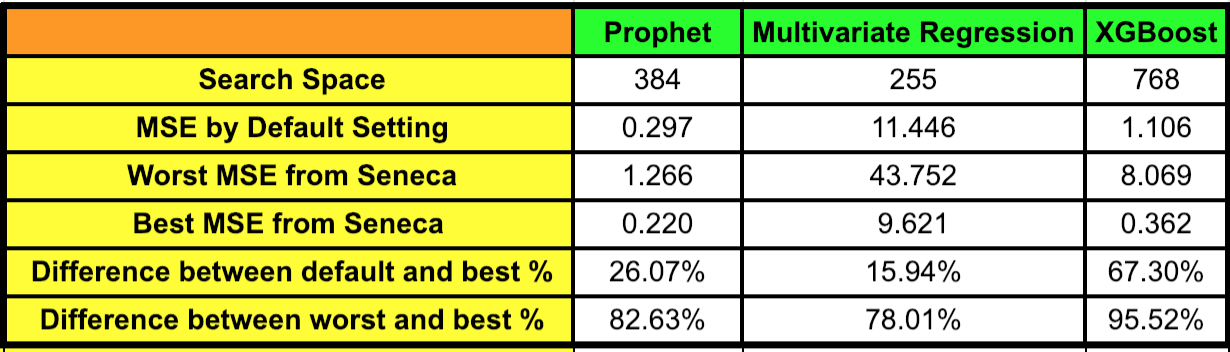
\includegraphics[scale=0.4]{mse}
\end{tabular}

\caption{Hyperparameter configuration count and MSE for the default, 
best (Seneca's recommendation), and worst configurations for the three regression applications. 
For the MSE  values (rows 3-5), lower is better.
\label{tab:mse}}
\vspace{-0.2in}
\end{table}

\begin{figure}[t] \centering 
\vspace{-0.5in}
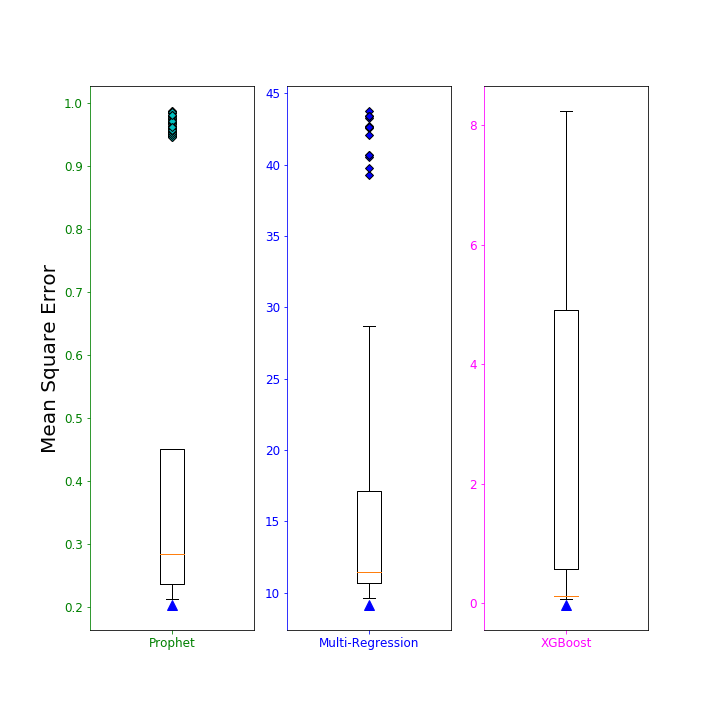
\includegraphics[scale=0.36]{box_plot_mse}
\caption{Box plot of MSE from the three regression applications across the 
hyperparameter tuning search space. The red notch shows the MSE from the default settings. 
The colored diamonds are outliers beyond two interquartile ranges. 
Seneca selects the points indicated by blue triangle.
Lower MSE values are better. 
\label{fig:box_plot_mse}}
\vspace{-0.2in}
\end{figure}

We first evaluate the quality of the output generated by each
ML applications when Seneca determines the hyperparameter settings. We
first show the results for the regression applications in
Table~\ref{tab:mse}.
The first row of data is the number of hyperparameter 
configurations that Seneca considers for each.
The last three rows show the MSE for the default, worst, and best performing (Seneca's recommendation)
hyperparameter configuation (lower is better).
Seneca reduces MSE by 22.56\%, 15.94\%, and 44.88\%, for Prophet, Multi-Regression, and XGBoost,
respectively, for the datasets and training methodologies that we consider.
Verses the worst case, Seneca reduces MSE by 82.62\%, 78.01\%, and 99.28\%, respectively.

Figure~\ref{fig:box_plot_mse} shows the MSE box plot for the hyperparameter search space for these applications (lower is better). 
The central rectangle covers the interquartile range (IQR),
which is defined as the range of data
points from first quartile to third quartile \texttt{$(Q3 - Q1)$}.
The upper whisker extends to the last datum less
than \texttt{$(Q3 + 2 * IQR)$} and the lower whisker extends to the first datum greater
than \texttt{$(Q1 - 2 * IQR)$}. The data points beyond the whiskers are considered outliers
and are plotted as colored diamonds. The red notch identifies the MSE that results from training
the model using the default settings of hyperparameter.
The blue triangle identifies the MSE of Seneca.
The difference between red notch and blue triangle
is the improvement brought about by the use of Seneca, over 
using the default parameter setting.
The plot also shows
that Prophet and Multi-Regression have a significant number of outliers,
indicating that a comprehensive search is critical to finding the best configurations.

%%%%%%%%%%%%%%%%%%%%% classification apps - ML model output quality %%%%%%%%%%%%%%%%%%%%%%%%%
\begin{table}
\centering

\begin{tabular}{|l|c|c|c|}
\hline
\textbf{80\%-20\%} & XGBoost & SVC & NN\\
\hline
\# of Combinations & 768 & 512 & 432 \\
\hline
\hline
Default Accuracy & 95.65\% & 21.77\% & 79.53\%\\
\hline
Worst Accuracy&0.00\%&14.08\% & 19.40\%\\
\hline
Best Accuracy (Seneca) &98.11\% & 40.81\% & 83.31\%\\
\hline
%\hline
%\hline
%\textbf{20\%-80\%} & XGBoost & SVC & NN\\
%\hline
%Default Accuracy & 95.07\% & 21.31\% & 55.44\%\\
%\hline
%Worst Accuracy&0.00\% & 9.42\% & 19.55\%\\
%\hline
%Best Accuracy (Seneca) & 98.68\% & 43.61\% & 60.89\%\\
%\hline
%\hline
%\textbf{0.1\%-99.9\%} & XGBoost & SVC & NN\\
%\hline
%Default Accuracy & 86.37\% & 20.02\% & 20.00\%\\
%\hline
%Worst Accuracy & 0.00\% & 19.99\% & 19.79\%\\
%\hline
%Best Accuracy (Seneca) & 89.14\% & 55.79\% & 29.99\%\\
%\hline

%percent difference between default and best 83.65%, 83.84%, 79.83%
%percent difference between worst and best 86.07%, 85.73%, 84.63%
%\begin{figure}[t] \centering 
%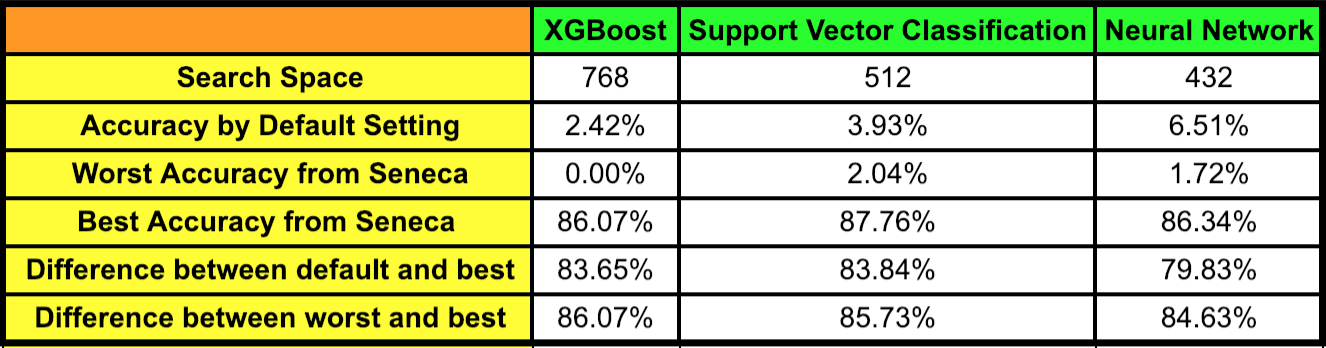
\includegraphics[scale=0.38]{accuracy}
\end{tabular}

\caption{Accuracy for the 
default, best (Seneca's recommendation), and worst hyperparameter configurations for 
the three classification applications using 80\% of the data to train and 20\%
of the data as a test set. Higher accuracy is better.
\label{tab:accuracy}}
\vspace{-0.1in}
\end{table}

\begin{figure}[t] \centering 
\vspace{-0.1in}
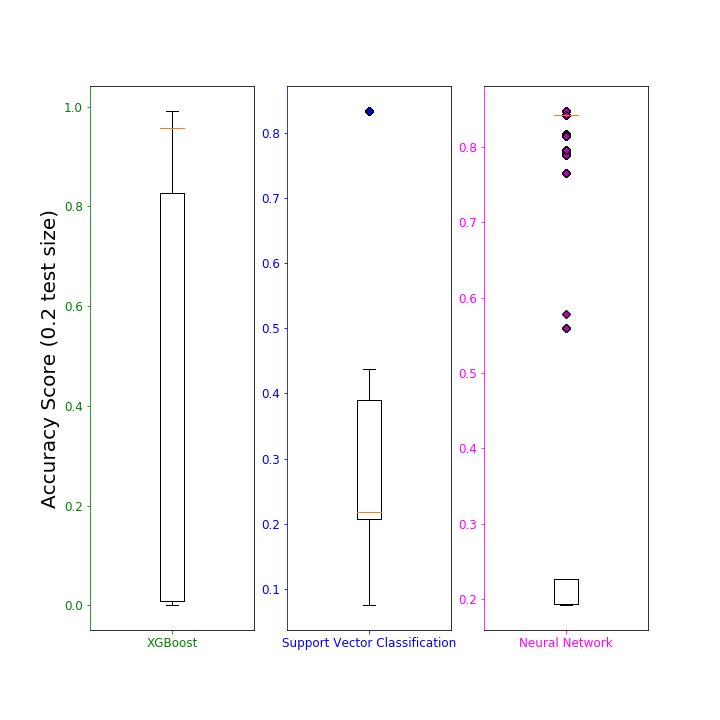
\includegraphics[scale=0.36]{box_plot_Accuracy_20}
\vspace{-0.4in}
\caption{Box plot of accuracy reported for three classification applications across 
the hyperparameter search space. The red notch indicates the accuracy that results
from default hyperparameter values.
The diamonds are outliers beyond two interquartile ranges. 
Seneca selects the points indicated by blue triangle. 
Higher accuracy is better. 
\label{fig:box_plot_accuracy}}
\vspace{-0.2in}
\end{figure}

\begin{table}[t]
\centering
\scriptsize
% \scriptsize
% \resizebox{\columnwidth}{!}{

\begin{tabular}{|l|c|c|c|} 
\hline
 & \textbf{Exec Time (Secs)} & \textbf{Memory Use (MB)} & \textbf{Best Accuracy}\\
\hline
\hline
XGBoost\_1 & 1244.42 (32.58) & 228.74 (15.92) & 99.13\% \\
\hline
XGBoost\_2 & 1280.56 (38.47) & 225.10 (19.67) & 97.70\% \\
\hline
SVC\_1 & 116.73 (1.11) & 224.44 (19.64) & 40.81\% \\
\hline
SVC\_2 & 115.33 (3.96) & 228.55 (16.20) & 44.11\% \\
\hline
NN\_1 & 116.10 (6.05) & 328.84 (16.40) & 83.31\% \\
\hline
NN\_2 & 121.29 (2.18) & 327.57 (16.44) & 83.92\% \\
\hline

\end{tabular}
%}

\ignore{ %the below has errors
% \scriptsize
% \resizebox{\columnwidth}{!}{

\begin{tabular}{|l|c|c|c|} 
\hline
 & \textbf{Exec Time (Secs)} & \textbf{Memory Use (MB)} & \textbf{Best Accuracy}\\
\hline
\hline
XGBoost\_1 & 1244.42 (32.58) & 228.74 (15.92) & 99.13\% \\
\hline
XGBoost\_2 & 1280.56 (38.47) & 225.10 (19.67) & 97.70\% \\
\hline
SVC\_1 & 116.73 (1.11) & 224.44 (19.64) & 40.81\% \\
\hline
SVC\_2 & 115.33 (3.96) & 228.55 (16.20) & 44.11\% \\
\hline
NN\_1 & 116.10 (6.05) & 328.84 (16.40) & 83.31\% \\
\hline
NN\_2 & 121.29 (2.18) & 327.57 (16.44) & 83.92\% \\
\hline

\end{tabular}
%}
}

\caption{The mean and standard deviation (in parentheses) for execution time and memory use 
(across 30 runs),
and best accuracy score for the classification applications using two different random splits. 
\label{tab:exec_memory}}
\vspace{-0.1in}
\end{table}


We next empirically evaluate Seneca's model output quality for the three
classification applications: XGBoost (classification), SVC, and NN.
Table~\ref{tab:accuracy} presents the accuracy percentage (higher is better)
for each application (3 right-most columns)
for the default, worst, and best (Seneca's recommendation) hyperparameter tuning
configurations (data rows 2-4).
The first row 
reports the number of configurations that Seneca considers in its search space.
Using a random 80/20 (train/test) percent split,
Seneca increases accuracy by 2.46\%, 19.04\%, and 3.79\%, for XGBoost
(classification), SVC, and NN applications, respectively.  
Because XGBoost and NN use a well-tuned default parameter set that works well for most datasets, Seneca provides only modest improvements.
Compared to the worst case however, Seneca improves accuracy by 98.11\%, 26.74\%, and 64.17\%,
respectively.  

Figure~\ref{fig:box_plot_accuracy} presents the accuracy box plot across the hyperparameter search space for these applications (higher is better).  
The central rectangle covers the first-third quartile
\texttt{$(Q3 - Q1)$} and the whiskers span from \texttt{$(Q3 + 2 * IQR)$} to \texttt{$(Q1 - 2 * IQR)$}.
The red notch indicates the accuracy metric from the model trained using the default
settings and colored diamonds show outliers beyond the whiskers.
The blue triangle at the top identifies the accuracy percentage reported by Seneca.

The model output quality results across applications, show that prediction
accuracy (for a given dataset) is dramatically
affected by hyperparameter settings.  Predictably, the default settings are
near the ``good'' end of the spectrum, however, Seneca is able to find the
parameterization that improves output quality over the default settings
in each case.

To investigate the potential impact of Seneca's 80/20 percent data split for the classification
applications, we next evaluate the quality of the output generated from 
each when we consider different 80/20 random splits.
To enable this, we run Seneca 30 times to obtain execution time, memory use, 
and best accuracy score. We report the
mean and standard deviation (in parentheses) 
for execution time and memory use across runs,
and the best accuracy score in
Table~\ref{tab:exec_memory}. Each pair of rows shows the results for two different random splits.
Our earlier results use input 1; this table adds results for a second, 80/20 
random split of the input (we also considered other random splits, which we omit for brevity, 
and the results are similar).  The performance and Seneca score is similar across splits. 
This result indicates that for these applications, 
users can repeatedly employ the recommended models for inference on other datasets or splits,
to amortize the cost of using Seneca.

\subsection{Cost Analysis}

We next analyze the monetary cost incurred by Seneca with and without 
Seneca's memory optimization.
We consider the use of the maximum allocatable memory (3GB) and Seneca's 
automatic detection and configuration of allocated memory.
This optimization requires
that Seneca intelligently probe to determine the best memory size 
to use.  We report the cost of these probes as \texttt{Optimizer Cost}.

Table~\ref{tab:cost_optimized} shows the results with and without
the Seneca memory optimization for each of the five applications.
The first two rows show the results when we use the maximum allocated memory 
for the Lambda functions. We present execution time in minutes (row 1) and 
monetary cost in cents (row 2). 
Rows 3--6 show the performance and cost when using Seneca's memory optimization.
\texttt{Exec time opt} is the execution time in minutes.
\texttt{Optimizer Cost} is monetary cost in cents of Seneca's memory size detector.
\texttt{Cost opt} is monetary cost in cents of using Seneca's memory optimizer.
\texttt{Total cost} is the overall cost of using Seneca to perform hyperparameter 
tuning for these applications and datasets (sum of Optimizer Cost and Cost opt).
The last two rows show the monetary savings in cents (row 7) and percent savings (row 8)
of using Seneca's memory optimization.  Seneca's memory optimization reduces
the monetary cost of its use from 10--35\% (25\% on average).


\begin{table}
\centering
\scriptsize
\resizebox{\columnwidth}{!}{
\begin{tabular}{|l|c|c|c|c|c|}
\hline
& \textbf{Prophet} & \textbf{MR} & \textbf{XGBoost} & \textbf{SVC} & \textbf{NN} \\
\hline
\hline
Exec time max (mins)& 24.96 & 4.18 & 17.48 & 1.91 & 2.49 \\
\hline
Cost max (\$) & 0.722 & 0.121 & 0.5 & 0.023 & 0.072 \\
\hline
\hline
Exec time opt (mins)& 38.7 & 8.72 & 29.07 & 1.95 & 3.17 \\
\hline
Optimizer Cost (\$) &0.033 & 0.014 & 0.003 & 0.010 & 0.008 \\
\hline
Cost opt (\$) &0.62 & 0.086 & 0.354 & 0.007 & 0.056 \\
\hline
Total Cost (\$) &0.653 & 0.1 & 0.357 & 0.016 & 0.064 \\
\hline
\hline
Savings (\$) & 0.07 & 0.02 & 0.15 & 0.007 & 0.008\\
\hline
Savings (\%) & 10\% & 17\% & 30\% & 30\% & 11\%\\
\hline
\end{tabular}
}

\caption{Seneca Memory Optimization: Rows 1--2 show the execution time and  monetary cost 
of using Seneca without its memory optimization (allocated memory = 3G). 
Rows 3-6 is the execution time and cost, 
respectively, when using the Seneca memory optimizer. 
Rows 7-8 show the savings in cents and percentage, respectively.
\label{tab:cost_optimized}}
%\vspace{-0.1in}
\end{table}

Table~\ref{tab:cost_optimized} illustrates two important points.
First, using AWS Lambda, full hyperparameter space exploration is inexpensive in
\textit{absolute} dollar cost terms and Seneca's automatic memory size optimization
decreases this cost further.  Second, memory optimization reduces cost but can 
increase the total execution time for parameter search 
since the functions must operate under additional memory 
constraints (versus using the maximum allocated memory).  
In addition, this cost fluctuates depending on the quality of the Lambda
execution environment (number of CPUs, Linux container overhead, 
multitenency, etc.).  We omit this data due to space constraints but analyze it here.
The average absolute difference in cost
across the five applications (30 runs) is \$0.05. %I use only split 1 for all 5
%numbers are below
Moreover, we have verified that the highest cost of execution under 
optimized memory is still cheaper than the lowest cost of execution under maximum 
memory for all five applications.
%$	Ave Cost	Highest Cost	Lowest Cost	Diff (High - low)
%Prophet	0.215	0.294	0.178	0.116
%Multi_Reg	0.076	0.078	0.075	0.003
%SVC_1	0.015	0.015	0.015	0.001
%SVC_2	0.014	0.016	0.013	0.003
%XGBoost_1	0.586	0.632	0.510	0.122
%XGBoost_2	0.607	0.630	0.569	0.061
%NN_1	0.055	0.059	0.051	0.007
%NN_2	0.058	0.061	0.056	0.005

\begin{table}
\centering
\scriptsize
\resizebox{\columnwidth}{!}{

\begin{tabular}{|l|c|c|c|c|c|}
\hline
& \textbf{Prophet} & \textbf{Multi\_Reg} & \textbf{XGBoost} & \textbf{SVC} & \textbf{NN}\\
\hline
%Seneca exec time (secs) & 756.09 & 245.21 & 1744.26 & 124.64 & 183.40\\
%\hline
%Seneca total cost (\$) & 0.198 & 0.057 & 0.398 & 0.014 & 0.044\\
%\hline
EC2 exec time (mins)                        & 73.79 & 21.99 & 359.87& 7.74 & 15.92\\
%Seneca, for reference: Exec time opt (mins)& 12.60 & 4.09 & 29.07 & 2.08 & 3.06 \\
\hline
EC2 total cost (\$)                    & 0.083 & 0.042 & 0.25 & 0.042 & 0.042\\
%Seneca, for reference: Total Cost (cents) &19.83 & 5.74 & 39.81 & 1.43 & 4.44 \\
\hline
\hline
%Speedup (x) & 5.86 & 5.38 & 12.38 & 3.72 & 5.21 \\
%\hline
yield & 50.86 & 340.23 & 83.36 & 0.00 & 1875.56\\
ideal yield & 25.43 & 170.12 & 41.68 & 0.00 & 937.78\\
\hline
\end{tabular}
}

\caption{Seneca VS EC2 cost analysis. Execution time (mins) and cost (cents) for
executing the applications serially in EC2 (t2.medium).  
Rows 3--4 show yield -- the additional speedup that
Seneca can achieve for each additional dollar spent for these applications.
Yield for SVC is 0 (infinite) because Seneca costs less than EC2 in this case.
Ideal yield shows the yield when we execute the applications in parallel (assuming
2x perfect parallelism).
\label{tab:yield}}
\vspace{-0.1in}
\end{table}

Finally, we compare the cost of Seneca to AWS Elastic Compute Cloud (EC2) use. 
We measure the execution time of Seneca using the
least expensive EC2 instance type in which the applications will run
(t2.medium, which has 2 multi-tenant cores and 4GB of memory). 
Note that EC2 instances are charged for by the hour; Lambda charges 
are only imposed when functions execute. We execute the applications serially
using the instance.  For this setting, Seneca enables a speedup over EC2 
of 3.72x -- 12.38x (6.51x on average). Doing so, however, imposes an additional 
cost of \$0.01--\$0.15 over EC2 for all but SVC. 
Seneca costs \$0.03 less than EC2 for SVC (because SVC runs in significantly less than
the next hour boundary).

To further understand the relationship between Seneca speedup and cost when Seneca
is more expensive (but faster) than using EC2, we define \texttt{yield} as 
$Y=\frac{T_{ec}}{T_{sc}}/({C_{sc} - C_{ec}}) \,|\ if \,C_{sc} > C_{ec}$ where $T_{ec}$ and $T_{sc}$ are the execution time, $C_{ec}$ and $C_{sc}$ are the total cost of EC2 instance 
and Seneca, respectively.
For applications for which Seneca is cheaper (e.g. SVC), we report \texttt{yield} 
as $0.00$.  This metric reveals the amount of speed up that Senence can achieve 
for each additional dollar spent.  To understand the yield if we were to 
parallelize the EC2 deployment (perhaps a more ``fair'' comparison), 
we also estimate yield for perfect parallelism (2x in our case for 
the t2.medium).  

We present results for this yield metric in Table~\ref{tab:yield} for each of the applications.
Rows 1 and 2 show the average execution time (in minutes) and cost (in cents) 
from using EC2 for each.
Rows 3 and 4 show the Seneca yield (speedup/\$).
Row 3 shows yield for serialized execution in EC2 (t2.medium
instance) and row 4 shows estimated yield if we were to achieve perfect parallelism
(i.e. 2x) using the EC2 instance. On average across the four applications for which
EC2 is cheaper, Seneca achieves yield of 294 (assuming perfect parallelism in EC2). 
That is, Seneca is able to provide a speedup
of 294x on average, for each additional dollar spent for these applications.
We plan to compare Seneca cost and performance 
to other EC2 instances and the AWS Elastic Container Service
as part of future work.

Overall, given the AWS Lambda pricing model and its Lambda performance variability, 
Seneca is still able to find the sweet spot between cost 
and execution time. Thus Seneca can be used to trade off time-to-solution 
for cost as desired by users, to automatically evaluate the impact of hyperparameter settings for ML models.

